\chapter{Appendix}


\section{PBL} 

Problem Based Learning $(PBL)$ is a method to organize the group work which will help to approach the projects objectives. Collaboration in the group is a very important factor to get the project working as efficient and fluent as possible.
Therefore there has initially been put some work into a way to work and organize the project. By doing that in the beginning we will save important time later on.
First of all this is a group of 6 people so it is important to give different tasks to different people to keep it efficient. 

To make sure everyone know what is going on there will be a group meeting at least once a week. Usually there will be more. Here the group members presents their progress for each other and if there has been any problems, it will be discussed here. In these meetings there are one chair-person who needs to make sure that all the topics of the agenda is being discussed. Besides the chair-person there is a referent who writes the minutes-of-meeting. 

A supervisor meeting will be held at least once every two weeks. Again with a chair-person and a referent. Before the meeting the agenda and questions has been sent to the supervisors and afterwards the group will sent the minutes-of-meeting. The goal here is to show the supervisors that the project is moving in the right direction and to get the questions answered. Furthermore the group sends the documentation to get feedback regularly.

To organize the tasks between the group members the web-page Trello is used as a taskboard. All the tasks that should be done is written here and divided the sections "To do", "Doing", "Done". This makes sure that everybody can see which tasks is in progress and who are working on them. A time-plan has been develop using a Gantt chart (Figure \ref{gantt}), so there is a common agreement on which tasks should be done at first.              

\clearpage

%\newgeometry{left=3cm,bottom=0.1cm}
%\KOMAoptions{paper=A3, paper = landscape, pagesize}
%\addtolength{\hoffset}{-4.0cm}
%\addtolength{\voffset}{2.5cm}
%\recalctypearea

\begin{landscape}

\section{Gantt chart}


%\vspace{1cm}
\begin{figure}[htbp]
	\begin{center}
		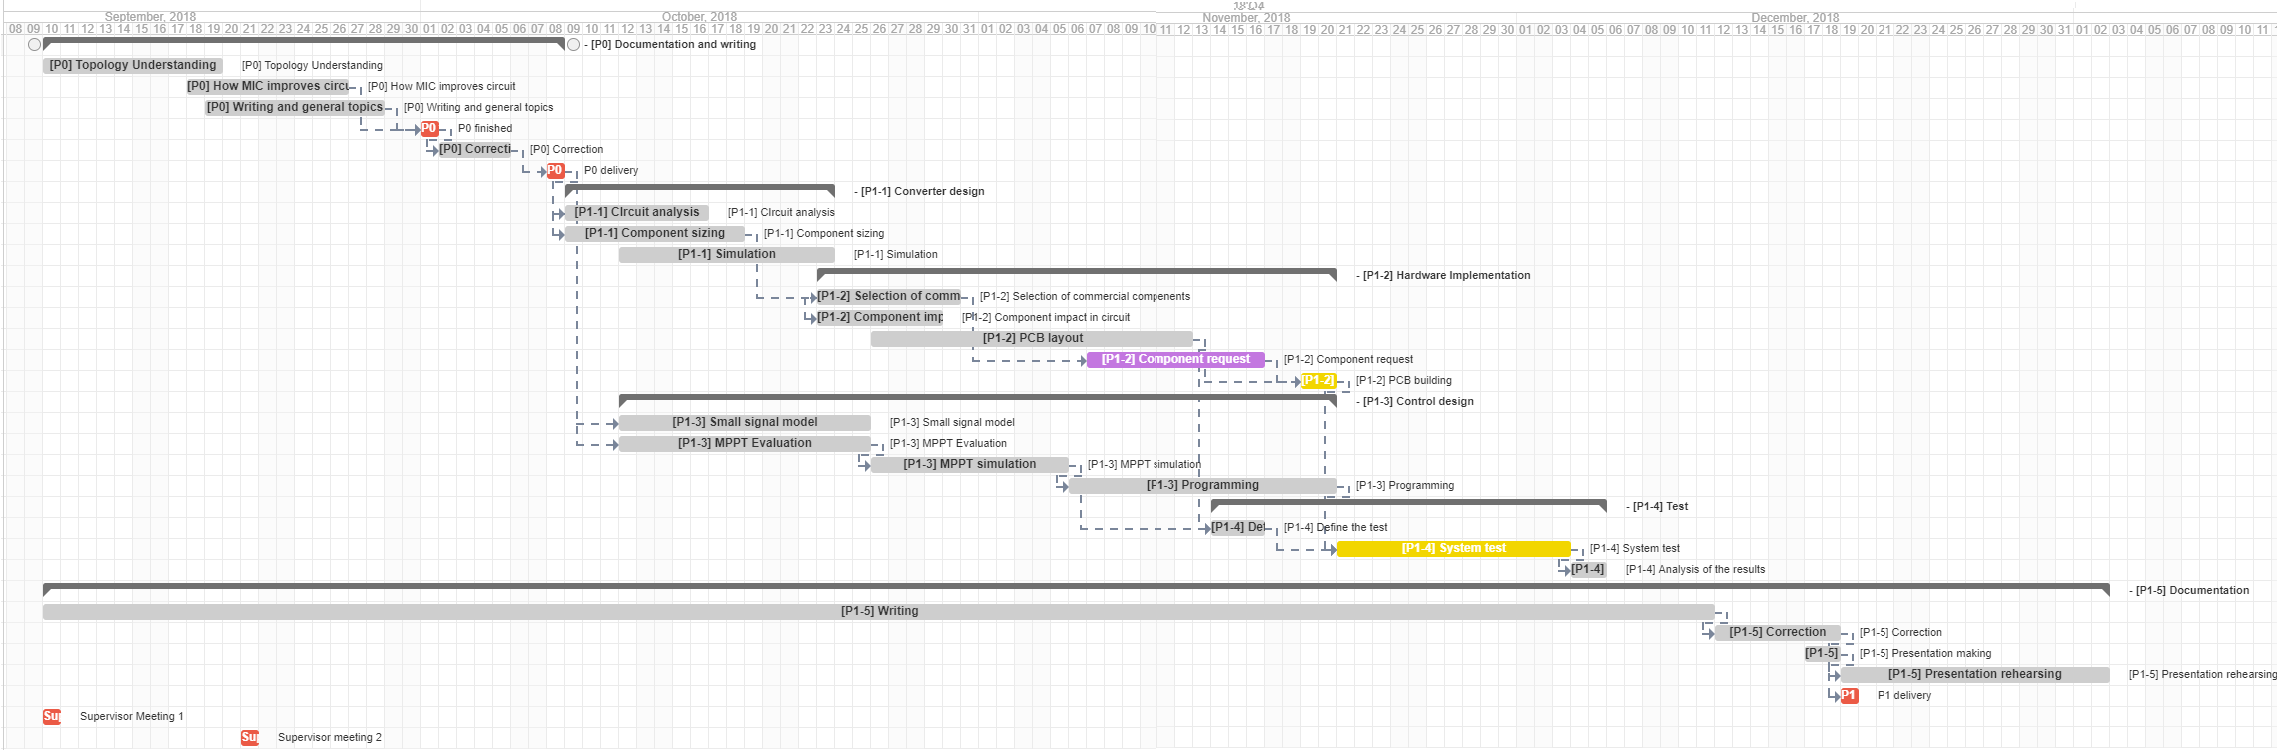
\includegraphics[width=1.6\textwidth]{../Pictures/Gantt_diagram_without_left_panel}
		\caption{Project Gantt chart}
		\label{gantt}
	\end{center}	
\end{figure}


\section*{Description of colors:}


\begin{table}[H]
	\centering
	\begin{tabular}{|p{3cm}|p{6cm}|} 
		\hline
		\textbf{Color} & \textbf{Description} \\ \hline
		Grey & Normal task  \\ \hline
		Red & Milestone  \\ \hline
		Purple & Supervisor interaction  \\ \hline
		Yellow &  Lab-work\\ \hline
	\end{tabular}
	\caption{Description of colors in the Gantt chart}
	\label{gantt_colors}
\end{table}

\end{landscape}
\clearpage
%\addtolength{\hoffset}{4.0cm}
%\addtolength{\voffset}{-2.5cm}
%\KOMAoptions{paper=A4, paper=portrait,pagesize}
%\recalctypearea


